\section{Model Selection and Assessment}
\textbf{Date:} \underline{Sep 9, 2025}

\subsection{Validation Sample}

\begin{figure*}[h]
    \centering
    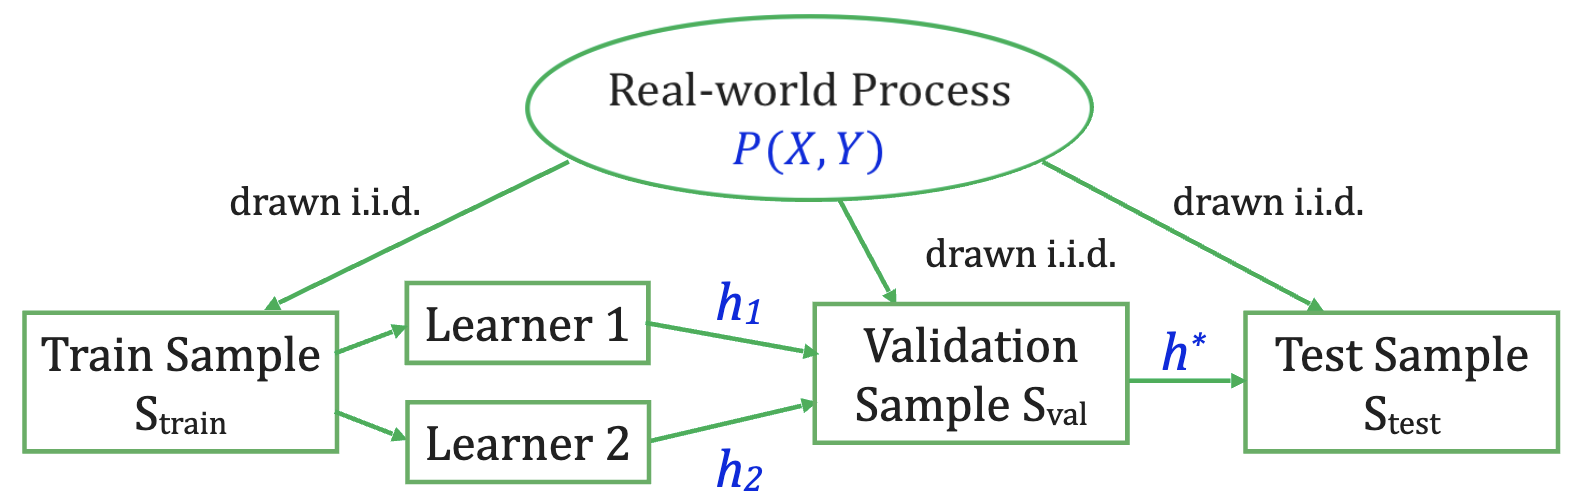
\includegraphics[width=0.8\textwidth]{Images/validation_sample.png}
    % \caption{Caption}
    % \label{fig:my_label}
\end{figure*}
\begin{itemize}
    \item \textbf{Training:} Run learning algorithm $l$ times (e.g. different parameters).
    \item \textbf{Validation Error:} Errors $err_{S_{val}}(h_i)$ are estimates of $err_{p}(h_i)$ for each $h_i$.
    \item \textbf{Selection:} Use $h^*$ with $\min\, err_{S_{val}}(\hat{h}_i)$ for prediction on test examples.
\end{itemize}

\paragraph{Two Nested Learning Algorithms}
\begin{itemize}
    \item \textbf{Primary Learning Algorithm on $S_{train}$}
    \begin{itemize}
        \item For each variant $A_1 \ldots A_l$ of learning algorithm, $h_i = A_i(S_{train})$
        \item Example: Decision Tree (DT) that stops at $i$ nodes.
    \end{itemize}
    \item \textbf{Secondary Learning Algorithm on $S_{val}$}
    \begin{itemize}
        \item Hypothesis space: $H' = \{h_1, \ldots, h_l\}$
        \item Learning Algorithm: $h^* = \arg\min\limits_{h \in H'} \left[ err_{S_{val}}(h) \right]$
    \end{itemize}
\end{itemize}

\paragraph{Typical ML Experiment}
\begin{itemize}
    \item Collect data $S = \left\{ \left( \vec{x}_1, y_1 \right), \ldots, \left( \vec{x}_m, y_m \right) \right\}$
    \item Split randomly into $S_{\text{train}}$, $S_{\text{val}}$, $S_{\text{test}}$
    \item REPEAT
    \begin{itemize}
        \item Train on $S_{\text{train}}$
        \item Validate on $S_{\text{val}}$
    \end{itemize}
    \item UNTIL we think we have a good rule $h$.
    \item Test $h$ on $S_{\text{test}}$ to evaluate its accuracy/error.
\end{itemize}

\subsection{Cross-Validation}
k-fold Cross-Validation:
\begin{itemize}
    \item \textbf{Given:}
    \begin{itemize}
        \item Training examples $S$
        \item Learning algorithm $A_p$ with parameter $p$ (model architectures or hyperparameters)
    \end{itemize}
    \item \textbf{Compute:}
    \begin{itemize}
        \item Randomly partition $S$ into $k$ equally sized subsets $S_1, \ldots, S_k$
        \item For each value of $p$:
        \begin{itemize}
            \item For $i$ from $1$ to $k$:
            \begin{itemize}
                \item Train $A_p$ on $S \setminus S_i$ and get $h_i$
                \item Apply $h_i$ to $S_i$ and compute $err_{S_i}(h_i)$
            \end{itemize}
            \item Compute cross-validation error:
            \[
                err_{CV}(A_p) = \frac{1}{k} \sum_i err_{S_i}(h_i)
            \]
        \end{itemize}
    \end{itemize}
    \item \textbf{Selection:}
    \begin{itemize}
        \item Pick parameter $p^*$ that minimizes $err_{CV}(A_p)$
        \item Train $A_{p^*}(S)$ on full sample $S$ to get final $h$
    \end{itemize}
\end{itemize}

\subsection{Generalization Error of Hypothesis}

\begin{itemize}
    \item \textbf{Given}
    \begin{itemize}
        \item Samples $S_{\text{train}}$ and $S_{\text{test}}$ of labeled instances
        \item Learning Algorithm $A$
    \end{itemize}
    \item \textbf{Setup}
    \begin{itemize}
        \item Train learning algorithm $A$ on $S_{\text{train}}$, result is $h$
        \item Apply $h$ to $S_{\text{test}}$ and compare predictions against true labels
    \end{itemize}
    \item \textbf{Test}
    \begin{itemize}
        \item Error on test sample $err_{S_{\text{test}}}(h)$ is estimate of true error $err_{p}(h)$
        \item Compute confidence interval
    \end{itemize}
\end{itemize}